\documentclass[a4paper,11pt]{article}
\usepackage{graphicx, amsmath, amssymb, geometry}
\geometry{margin=2cm}
\title{Resonanz-Äther Gravitation -- Kurzreport}
\author{[Dein Name]}
\date{\today}
\begin{document}
\maketitle
\section*{Zusammenfassung}
Wir vergleichen drei Modelle der Gravitation im Rahmen eines Resonanz--Äther-Ansatzes: 1×Exponential, 2×Exponential und ein Hybridmodell, das das Fernfeld $1/r^2$ exakt erzwingt und Nahfeldkorrekturen mittels Exponentials zulässt.

\section*{Ergebnisse}
RMSE (über $r\in[R,\,3R]$):
\begin{itemize}
\item 1×Exp: 3.404e-01 m/s$^2$
\item 2×Exp: 7.606e-03 m/s$^2$
\item Hybrid: 0.000e+00 m/s$^2$
\end{itemize}

\section*{Grafiken}
\begin{center}
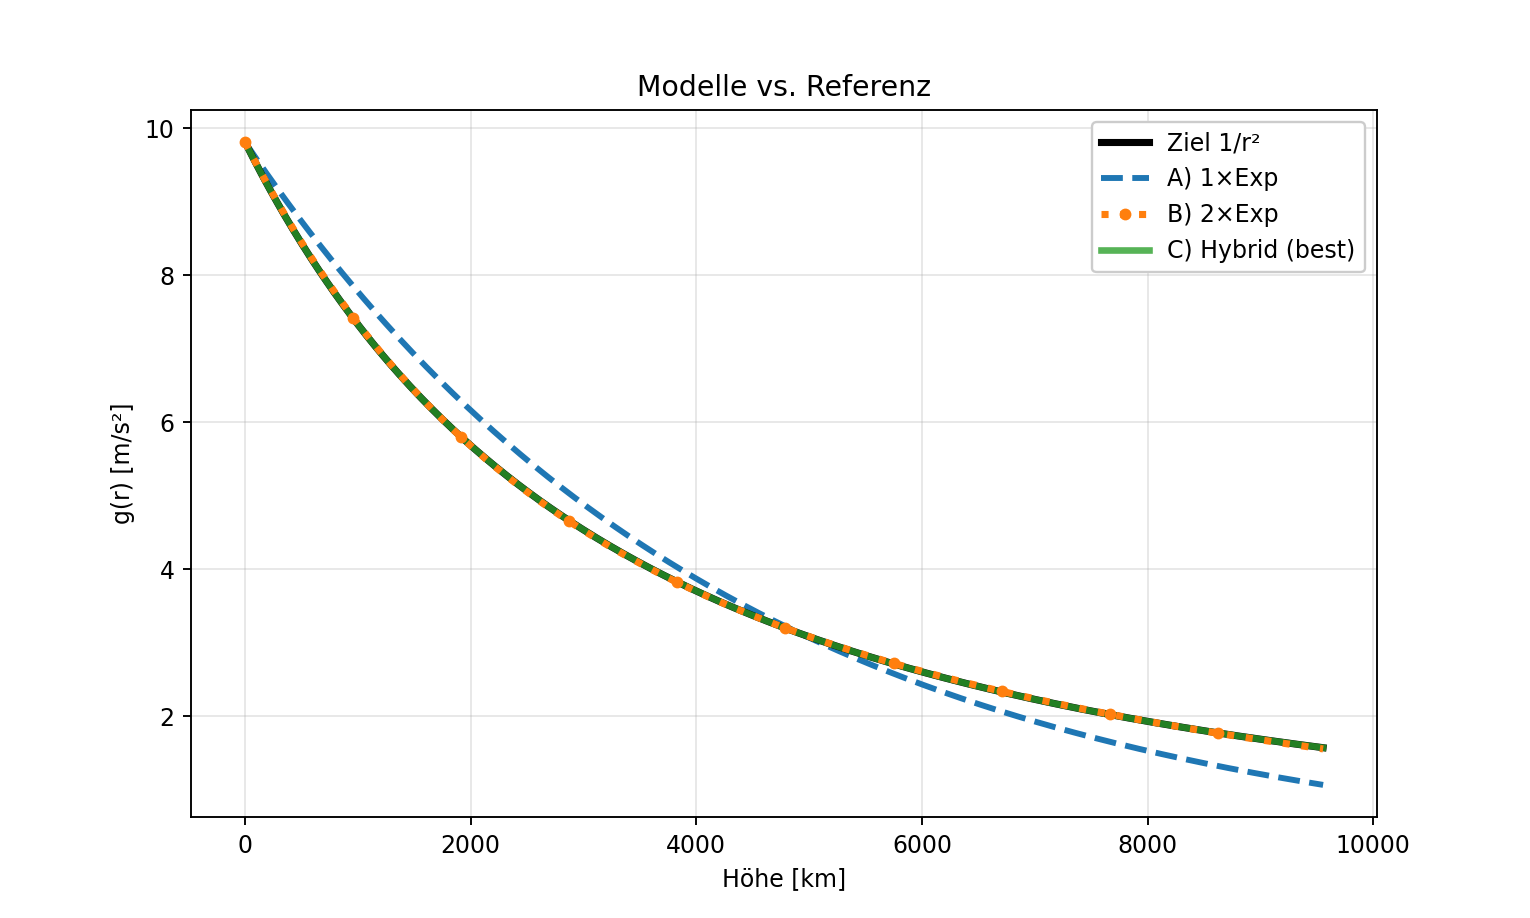
\includegraphics[width=0.95\textwidth]{profiles.png}\\
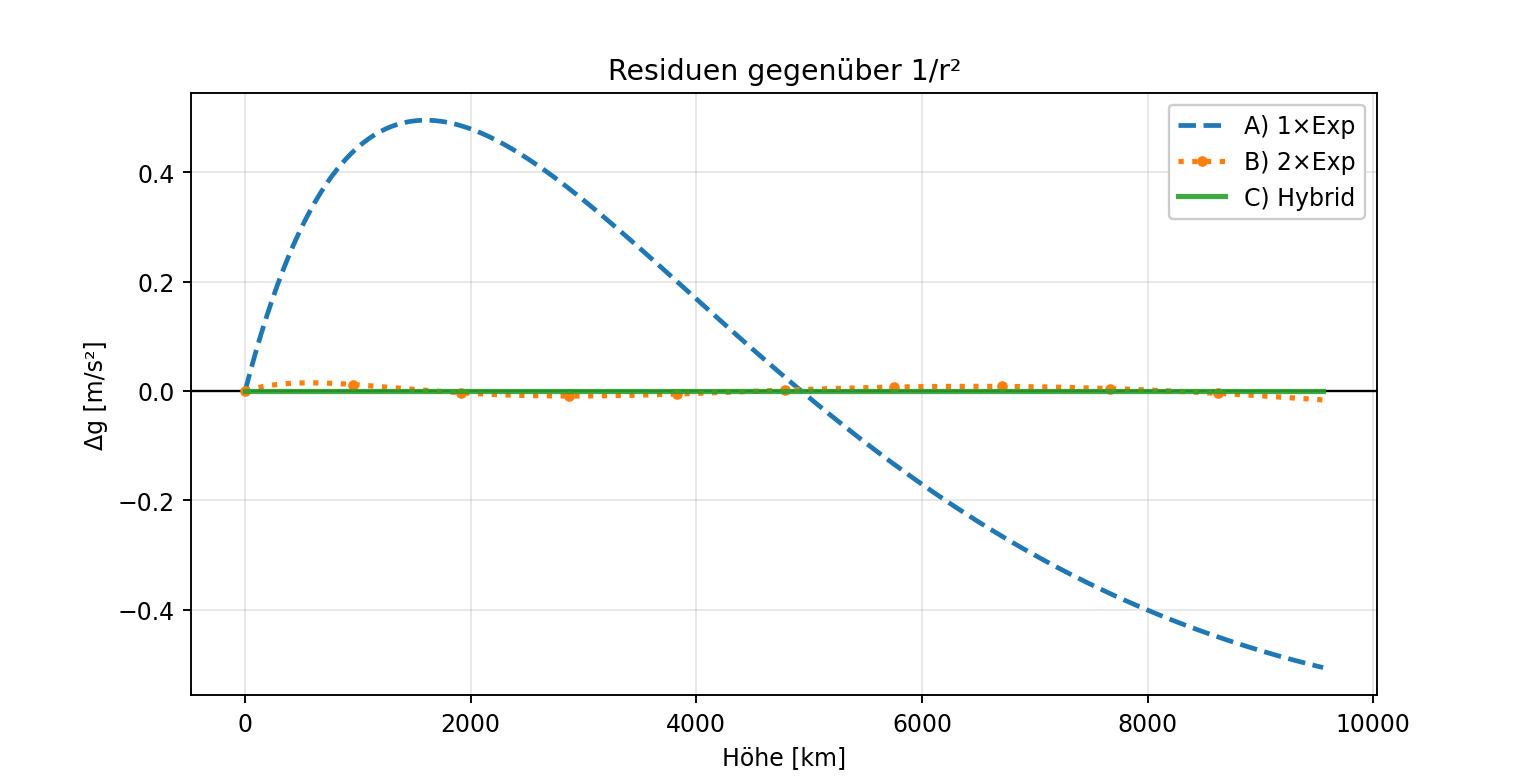
\includegraphics[width=0.95\textwidth]{residuals.png}\\
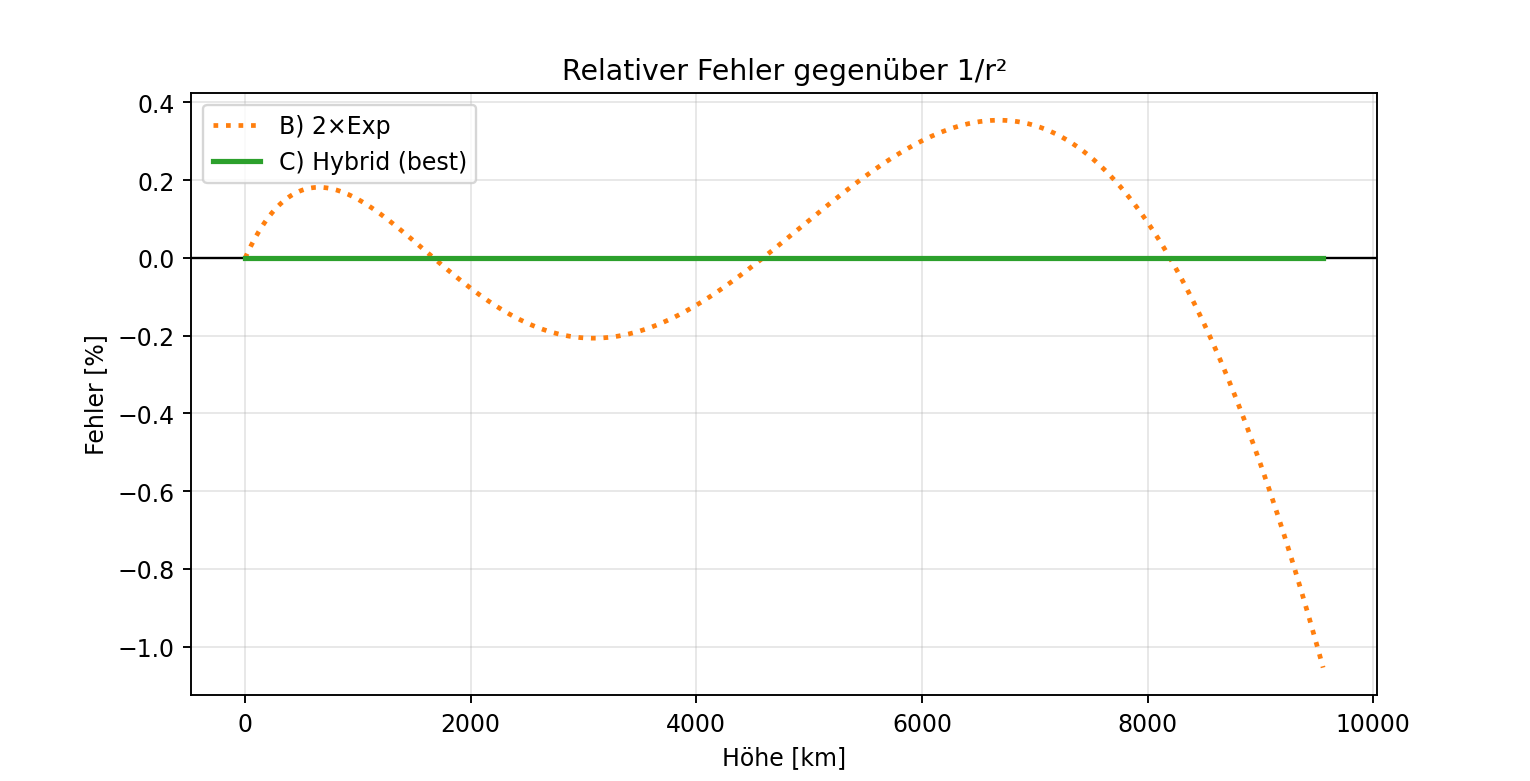
\includegraphics[width=0.95\textwidth]{percent_error.png}\\
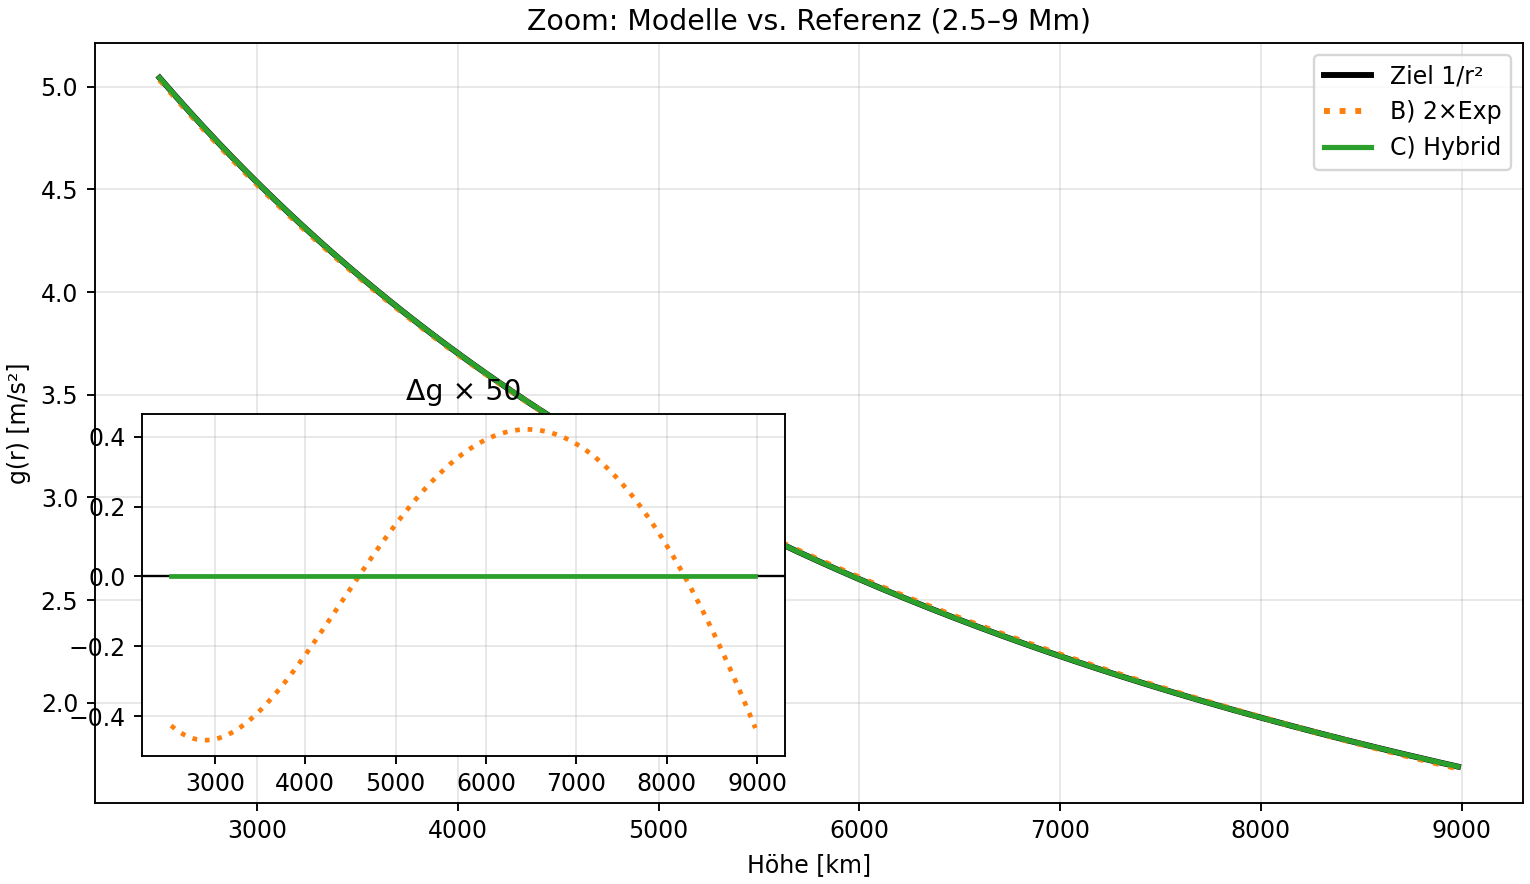
\includegraphics[width=0.95\textwidth]{zoom_delta.png}\\
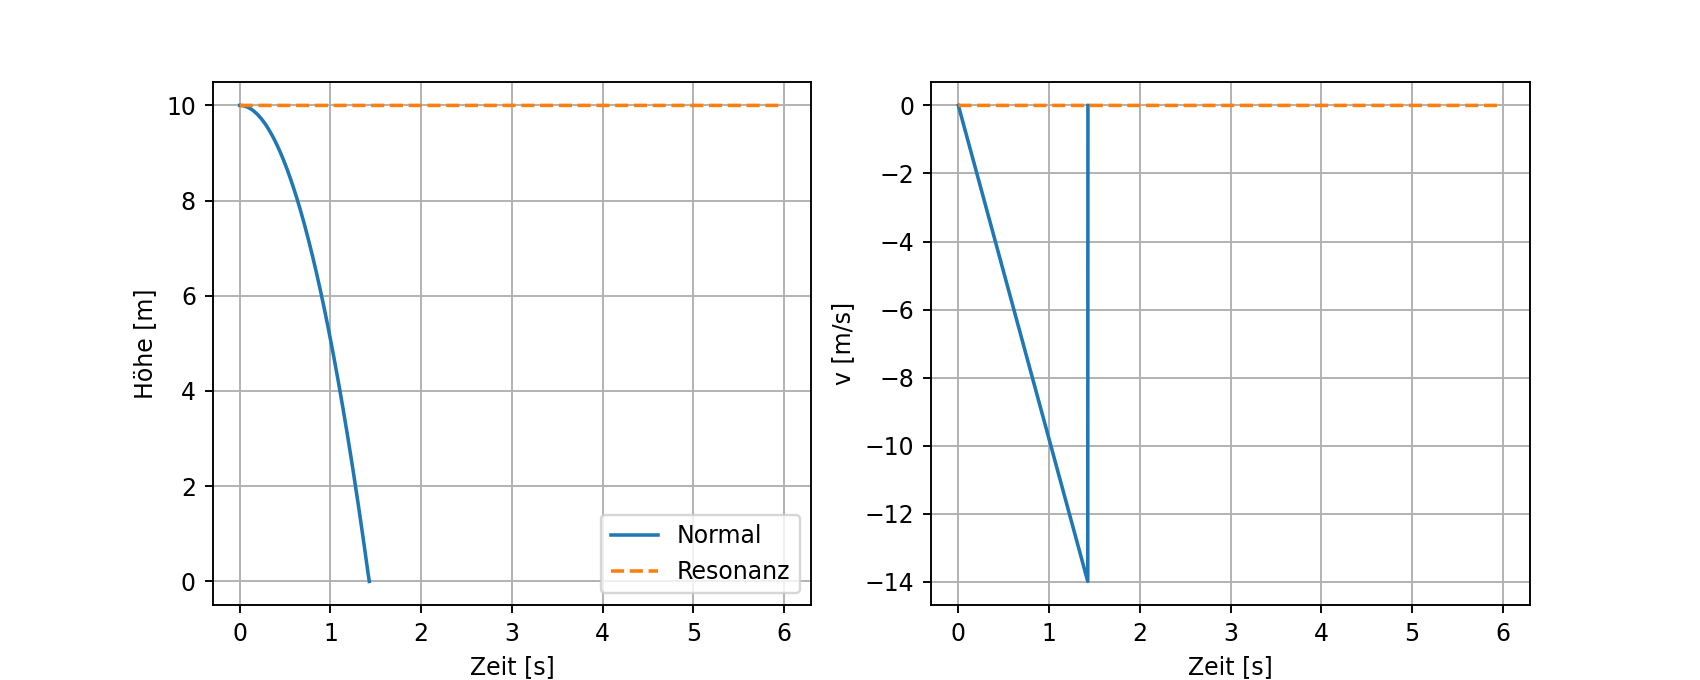
\includegraphics[width=0.95\textwidth]{drop.png}\\
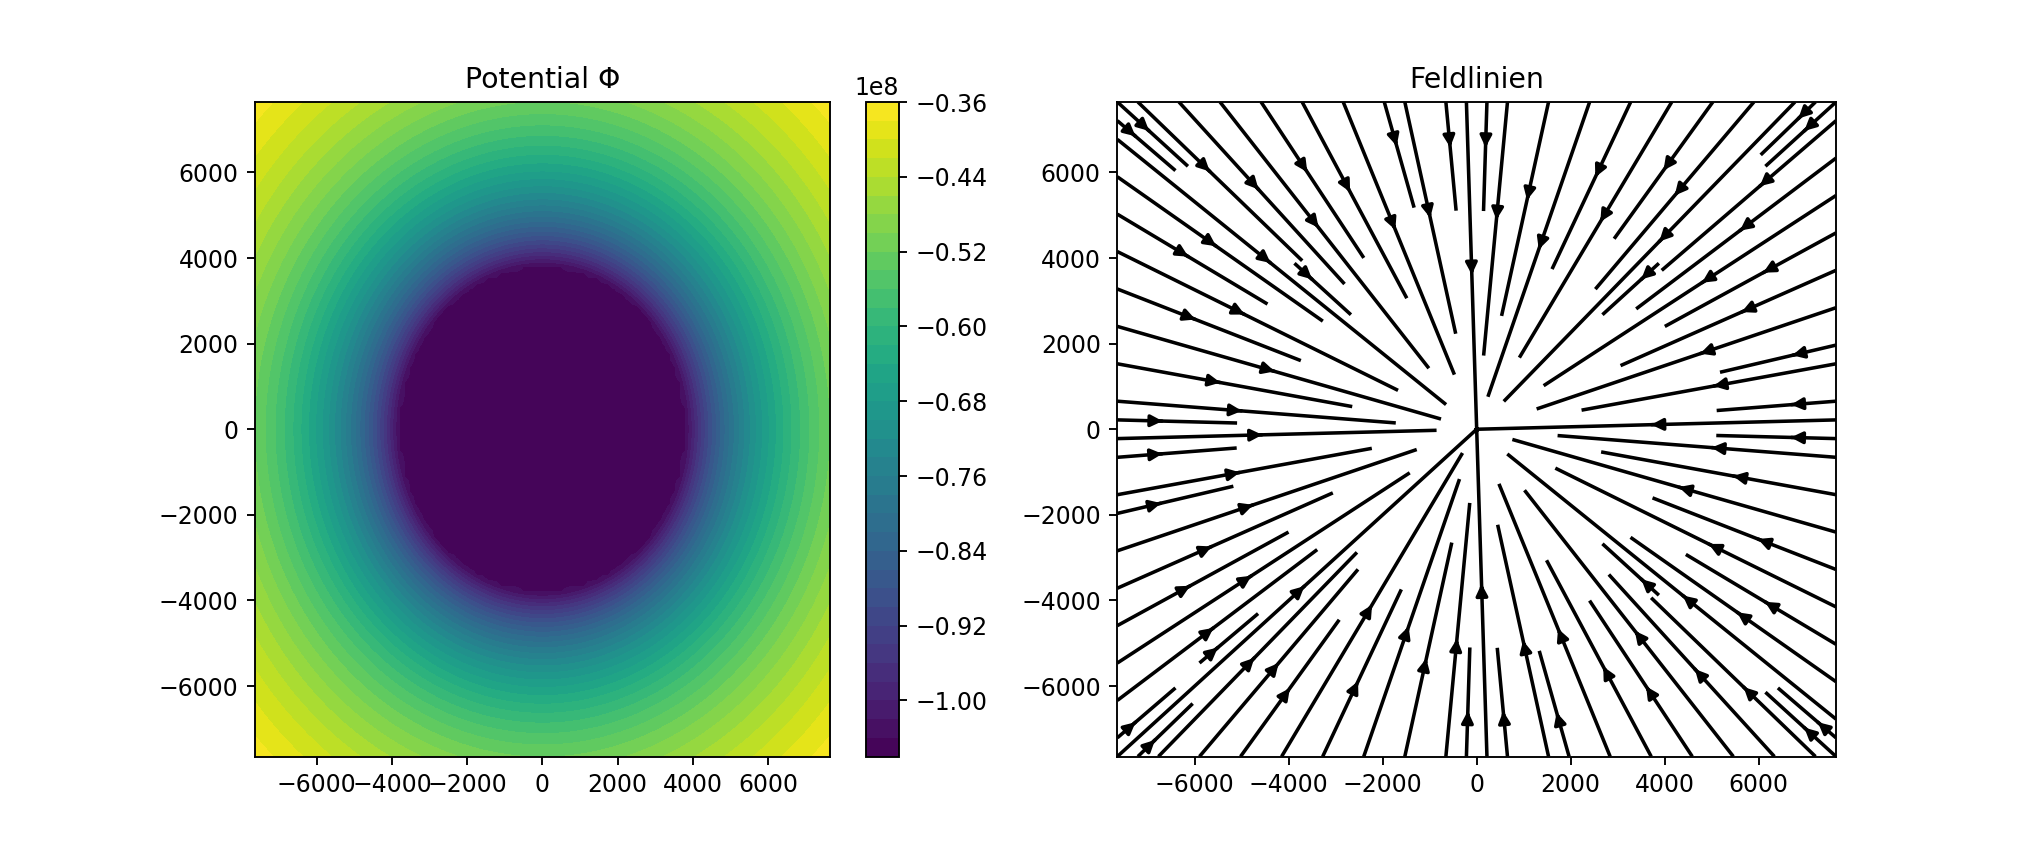
\includegraphics[width=0.95\textwidth]{field.png}
\end{center}
\end{document}
